\chapter{Introduction}
\label{chap:Int}

Since the invention of smart devices, the mobile traffic has been increasing tremendously over the last decade. According to the recent surveys on mobile traffic by prominent market leaders (Cisco \cite{CISCO14} and Ericsson\cite{Eric15}), the existing mobile traffic is expected to increase $11 \times$ by 2021. The wireless community including the standardization bodies (3GPP \cite{3GPP}) believe that the state-of-the-art standards (fourth-Generation (4G) -- LTE, WiMAX) are not capable of sustaining these ever-increasing demands in the upcoming decade. With this situation in hand, the standardization bodies are currently in the phase of conceptualizing the requirements of the fifth-generation (5G) of mobile wireless systems.
Some of these major requirements are: (i) areal capacity in $\SI{}{bits/sec/m^2}$ must increase by a factor of $1000$ compared to 4G, (ii) low latency of approximately \SI{1}{ms}, and, (iii) energy- and cost-efficient deployment \cite{Qual13, Andrews14}.
 %One of the major goals is to improve the areal capacity ($\SI{}{bits/s/m^2}$) by a factor of 1000 \cite{Qual13, Andrews14}. \tc{To this end, an extension to the already allocated spectrum is of paramount importance.} 
The feasibility of these requirements can be ensured by applying promising approaches such as maximization of the spatial degrees of freedom using Massive MIMO \cite{Lar14} and 3D-beamforming \cite{Hal13}, In-band full-duplex communications \cite{Sab14}, small cell densification \cite{Andrews12, Gel13}, alternatives to the already allocated spectrum using millimeter-Wave technology (mmW) \cite{Rapp13}, visible light communications \cite{Wu14}, and dynamic spectrum access to the licensed spectrum, a Cognitive Radio (CR), and waveform design \cite{Scha14, Baz15}, \figurename~\ref{fig:5G} describes a classification of these approaches. In order to narrow down the perspective, in this thesis, a deployment scenario that lays emphasis on the small cell densification and the implementation of cognitive radio techniques is proposed. Before moving any further, let us elaborate on the underlying facts that make these approaches or their combination suitable candidates for the 5G networks. 

\begin{figure}
\centering
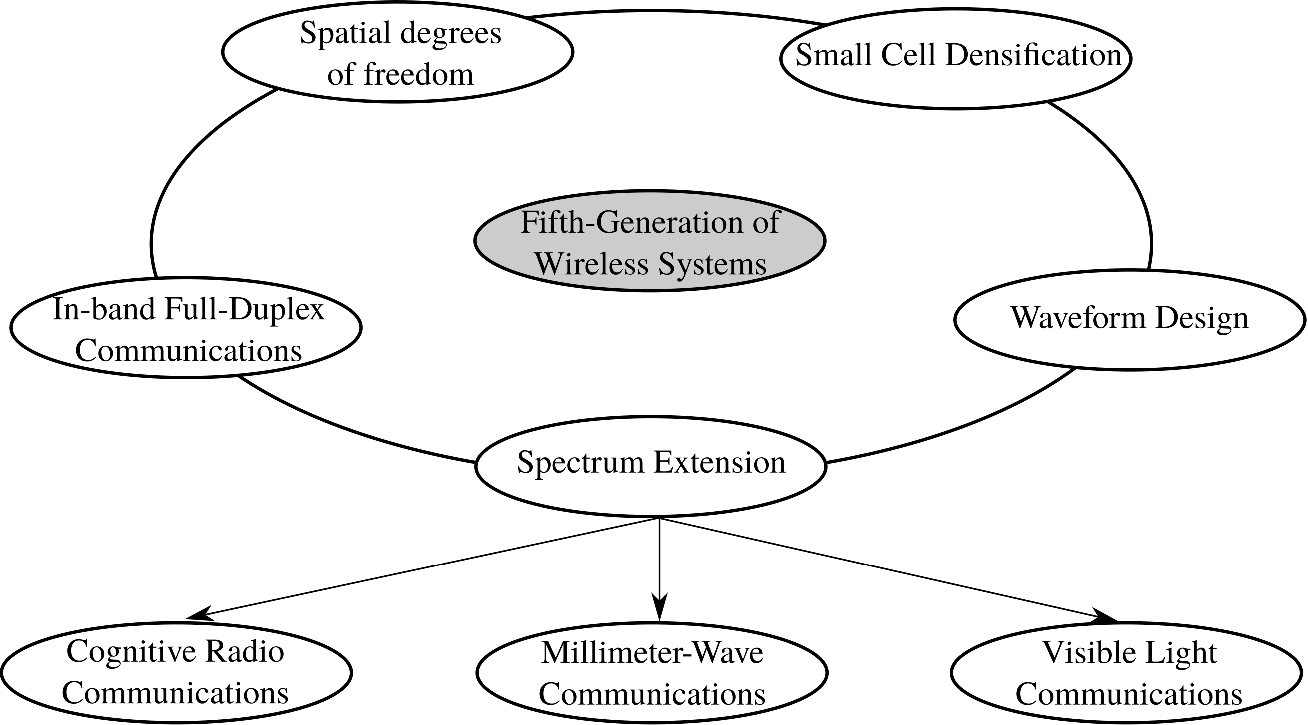
\includegraphics[width = 0.98 \columnwidth]{figures/5G}
\caption{An illustration of the possible candidates/techniques considered under the 5G framework.}
\label{fig:5G}
\end{figure}


\subsubsection*{Small Cell densification}

In the recent past, Small Cells (SCs) have emerged as a potential solution for coverage and capacity enhancements inside a wireless network. A SC represents a low power station that ranges from $\SI{10}{m}$ to $\SI{100}{m}$. The reduced transmit distance accomplished with the deployment of SCs enhances the link quality and aids spatial reuse \cite{Chander08}.
%SC is particularly deployed in a indoor or outdoor environments, these include enterprise, shopping complex or residential \cite{SSF14}. 
As a result, small cell densification can leverage the areal capacity of a 5G network \cite{Andrews14}. The capacity, however, increases linearly with the number of SCs, it is infeasible to procure the factor of $1000$ in the areal capacity with densification alone. Not only this, the operation and the integration of these substantial number of SCs to the backhaul network are cost- and energy-intensive for the mobile operator, which somehow limits the degree to which the densification can be achieved by a wireless network.





\subsubsection*{Spectrum extension}
Complementing the link quality by means of SCs, the spectrum represents a major contribution to the desired areal capacity. Given the present situation of the spectrum allocated to different mobile applications, it is difficult to procure an extension to the already allocated spectrum. Before investigating the potential candidates for the spectrum extension, it is necessary to consider the following classification of the spectrum:
%\begin{itemize}
(i) $\ge \SI{6}{GHz}$;
(ii) $\le \SI{6}{GHz}$.
%\end{itemize}
The prime objective of this sort of classification is to shift the focus on the propagation characteristics and the issues thereof.


The spectrum beyond \SI{6}{GHz} largely entails the millimeter Wave (mmW), which is well-known for point-to-point communications. Recently, it is envisaged as a powerful source of spectrum for 5G wireless systems. However, the millimeter wave technology is still in its initial stage and along with complex regulatory requirements in this regime, it has to address several challenges like propagation loss, low efficiency of radio frequency components such as power amplifiers, small size of the antenna and link acquisition \cite{Rapp13}. Therefore, in order to capture a deeper insight of its feasibility in 5G, it is essential to overcome the aforementioned challenges in the near future\nociteK{Kaushik13, Kaushik14_W, Kaushik14_CC, Kaushik14_P, Kaushik15_CC,Kaushik15_ICC, Kaushik15_D, Kaushik16_TWC, Kaushik16_VTC1, Kaushik16_TCCN, Kaushik16_ICC, Kaushik16_CC, Kaushik16_VTC2}

\begin{figure}[!t]
\centering
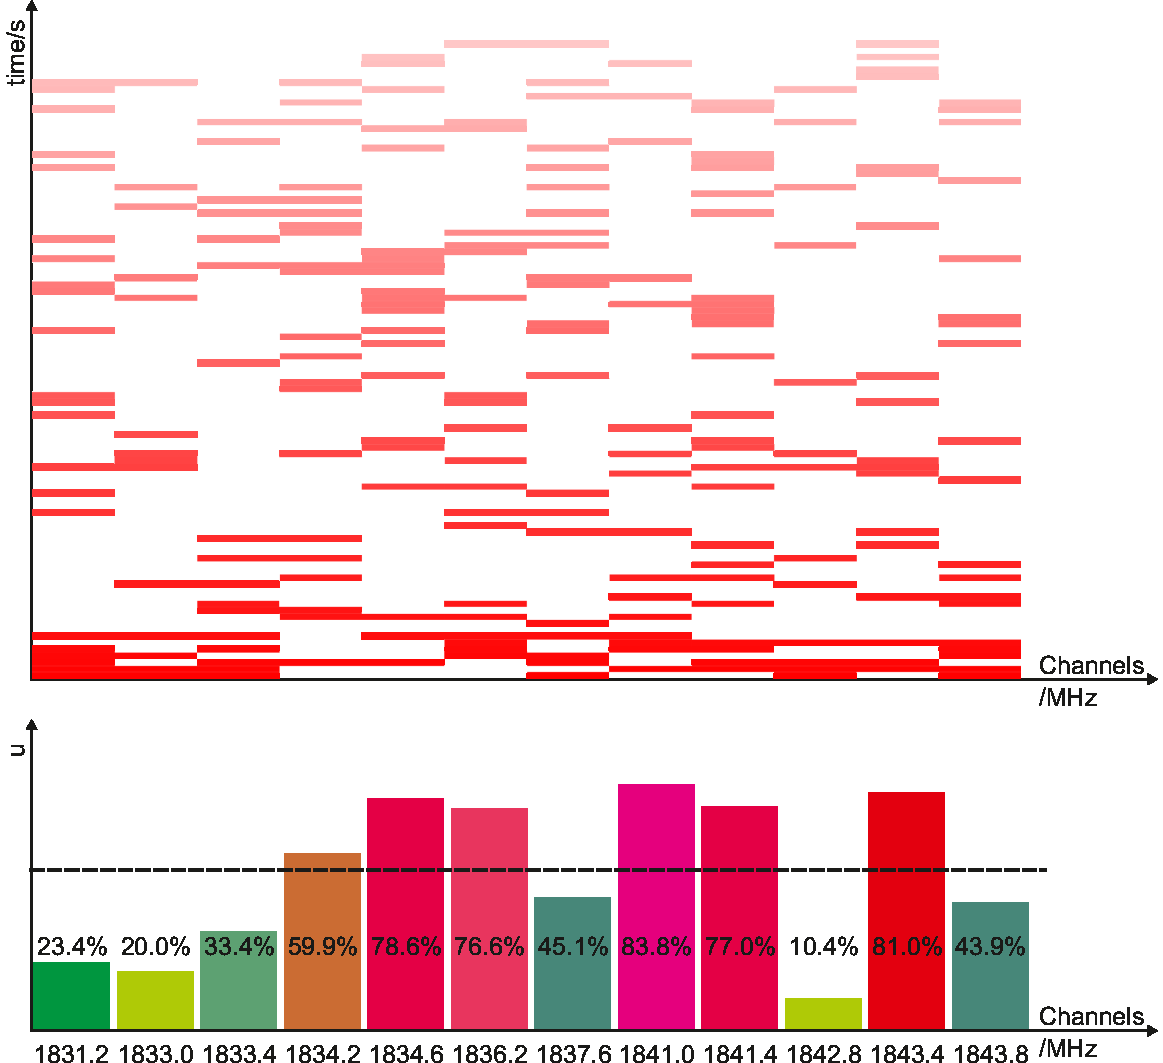
\includegraphics[width = 0.9\columnwidth]{figures/Grafik_Poster}
\caption{A snapshot of a hardware demonstrator that measures the spectral occupancy in GSM \SI{1800}{MHz} downlink channels, whereby the slices (red and white) represent the channel occupancy (1 or 0) corresponding to a single measurement at a given time instant. The bar plots illustrate the channel occupancy (u) for each channel with a history of 500 measurements\protect\citeK{Kaushik13}.}
\label{fig:HW_I}
\end{figure}


Besides the spectrum beyond \SI{6}{GHz}, an efficient utilization of the spectrum below \SI{6}{GHz} presents an alternative solution. The use of the spectrum in this regime (below \SI{6}{GHz}) is fragmented and statically allocated \cite{Mchen05, Mchen07}, leading to inefficiencies and the shortage in the availability of the spectrum for new services. To justify the statement that the spectrum is under-utilized, a glimpse of the measurement campaign conducted during the peak hours for determining the spectral occupancy for the GSM \SI{1800}{MHz} downlink channels is presented in \figurename~\ref{fig:HW_I}. Hence, the demand for the additional spectrum can be fulfilled only if we manage to utilize this radio spectrum efficiently. In this perspective, Cognitive Radio (CR) is foreseen as one of the potential contenders that addresses the spectrum scarcity problem. Since its origin by Mitola \textit{et al.} in 1999, this notion has evolved at a significant pace, and consequently has acquired certain maturity. Despite the existence of the theoretical analysis, from a deployment perspective, this technology is still in its preliminary phase \cite{Pawe11}. Due to this large gap between the theoretical models and practical implementations, recently, the wireless community has started to show an inclination towards models and/or techniques that enable the placement of this concept over a hardware platform so that the disposition of CR systems in the upcoming 5G wireless networks can be facilitated. Understanding the significance these facts, this thesis capitalizes on the deployment of the CR system. 


\section{Background and Motivation}
\label{sec:mot}

\subsubsection*{Cognitive Radio Systems}


In order to proceed further, it is essential to understand the classification of different CR systems described in the literature. An access to the licensed spectrum is an outcome of the paradigm employed by the \tc{Secondary User (SU)}. In this context, all CR systems that provide shared access to the spectrum mainly fall under the following categories \cite{Goldsmith09} (please consider \figurename~\ref{fig:paradigm} for a graphical illustration of different CR systems and their corresponding techniques): 
\begin{itemize}
\item According to Interweave Systems (ISs), the SUs render an interference-free access to the licensed spectrum by exploiting spectral holes in different domains such as time, frequency, space and polarization. 
\item Underlay Systems (US) enable an interference-tolerant access under which the SUs are allowed to use the licensed spectrum (e.g. Ultra Wide Band) as long as they respect the interference constraints of the Primary Receivers (PRs). 
\item Hybrid Systems (HSs) combine the benefits of the IS (agility to detect spectrum holes in different domains) and the US (interference-tolerant capability) to enhance the spectral usage efficiency.  
\item Overlay systems consider the participation of higher layers for enabling the spectral coexistence between two or more wireless networks. 
\end{itemize}
Since the IS, US are HS are closely associated with the physical layer, these systems are mostly considered not only for the theoretical analysis but for practical implementations as-well \citeK{Kaushik13,Kaushik14_CC,Kaushik15_D, Kaushik16_CC, Kaushik16_VTC2}, \cite{Cabric04, Cabric06, Kim10}. Taking this into account, the thesis focuses on the performance analysis of these CR systems from a deployment perspective. In order to illustrate the successful incorporation of a CR technique in a 5G network, a specific use-case (deployment scenario) is presented subsequently. 


\begin{figure}
\centering
\includegraphics[width = 0.85 \columnwidth]{figures/CR_paradigm}
\caption{A classification of different CR systems and their corresponding techniques that allow shared access to the licensed spectrum.}
\label{fig:paradigm}
\end{figure}



\subsection{Cognitive Small Cell: A Prominent Use-case}
\begin{figure}
\centering
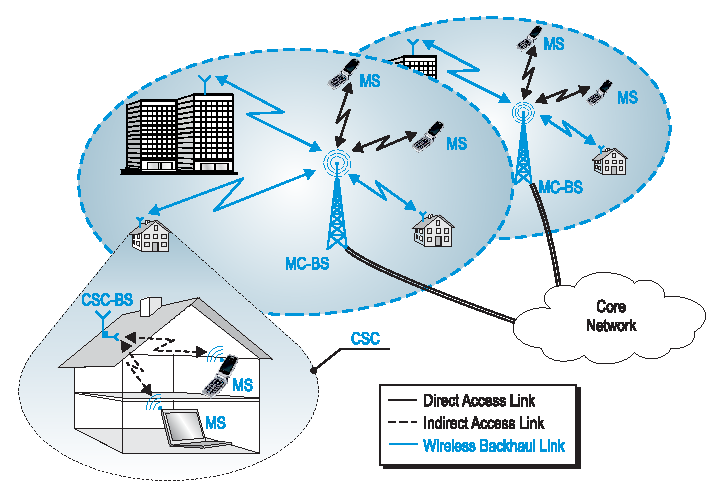
\includegraphics[width = 0.9 \columnwidth]{figures/Cellular_Scenario_CR6F}
\caption{An illustration of the CSC deployment in a 5G network.}
\label{fig:archi}
\end{figure}



Following the previous discussion, it is evident that spectrum extension via CR systems and SCs densification are key-enablers for the 5G system.
%Recently, ElSawy \textit{et al.} \cite{Elsawy13} have presented Cognitive Small Cell (CSC), a concept that fulfills the capacity demands of the future wireless networks. 
Based on this fact, a preliminary concept of Cognitive Small Cell (CSC), a promising application that combines the benefits from the SC deployment and the efficient usage of the spectrum below \SI{6}{GHz} by implementing CR techniques to accomplish the requirements of 5G networks is presented. A typical scenario where the CSC finds its application would be the co-existence of Wifi or unlicensed small cell and wireless cellular systems \cite{Benn13, Gali15}. The notion of CSC has been previously investigated by Elsawy \textit{et al.} \cite{Elsawy13, Elsawy13_cmag} and Wildemeersch \textit{et al.} \cite{Wild13}, where the authors primarily emphasized on the modelling techniques\footnote{The modelling is based on stochastic geometry, which allows a spatial averaging over multiple network geometries \cite{Haenggi, Haenggi08now}.} that depict the positioning of several CSCs inside the network. Due to this, the performance analysis of the CSC has been limited mainly to network abstraction. In contrast, this thesis emphasizes on key-aspects encountered while deploying a CSC, which otherwise could forbid its realization on a real hardware. %, which could possibly lead to a successful integration of CSCs in the 5G network. %Consequently, by considering different CR paradigms to enable secondary usage of the licensed spectrum, here a deeper comprehension of the concept is illustrated. %, thereby, making it accessible to 5G systems. 
%To strengthen our understanding of CSC, we demonstrate the feasibility of the respective paradigms by means of hardware implementations.
%Pertaining to the deployment, we analyze the true performance of the CSC as a CR application for the mentioned paradigms.  
 A comprehensive incorporation of CSC in a preliminary 5G architecture is illustrated in \figurename~\ref{fig:archi}. In order to enhance the viability of the proposed network architecture, it is interesting to highlight some of the essential ingredients pertaining to the deployment of the CSC.

\subsubsection*{Network Elements}
 In order to propose a successful integration of CSC in a 5G network, the following key elements are essential: a CSC-Base Station (CSC-BS), a Macro Cell-Base Station (MC-BS) and Mobile Stations (MSs), cf. \figurename~\ref{fig:archi}. MSs are the devices either served by the MC-BS over a \textit{direct access} link or the CSC-BS over an \textit{indirect access} link. The direct access and the indirect access are the nomenclature used to distinguish a start-of-the-art (spectrum) access between the MC-BS and the MS from an access between the CSC-BS and the MS representing a CR communication, respectively. Furthermore, the MC-BS is connected to several CSC-BSs over a \textit{wireless backhaul} link. Although the MC-BS and the MS already exist in the conventional cellular architecture, to incorporate the opportunistic access inside the CSC, it is necessary to consider a functionality upgrade.

\subsubsection*{Spectrum Access}
In the proposed network architecture, the access to the spectrum is realized over the wireless backhaul, the direct access and the indirect access links, cf. \figurename~\ref{fig:archi}.
\begin{enumerate}
\item A wireless backhaul is a
%quasi-line of sight\footnote{It allows limited number of objects between the direct link.} 
point-to-point wireless link between the CSC-BS and the MC-BS that relays the traffic generated from the CSC to the core network. Accounting the desification of the CSC in 5G network, the wireless backhaul link, in contrast to the optical fiber link, presents a cost-effective and energy-efficient alternative to the mobile operator.
With the limited infrastructure required for deployment, it accelerates the installation process and promotes scalability of the network.
For the wireless backhaul link, an exclusive spectrum for a longer duration is desired. Hence, it is sensible to nominate a mmW band; alternatively, an exclusive band below \SI{6}{GHz} can be acquired using the principles of Licensed Shared Access \cite{ETSI13}.
%These WB links encourage ultra-densification as they brings down the capital expenditure and offer scalability to the vendor. 

\item A direct access link represents a direct access of the MS at the MC-BS over the allocated spectrum. Consequently, the spectrum access for this link is analogous to the one existing in the state-of-art wireless standards.
\item The CSC elements (the CSC-BS and the MS) are responsible for executing the secondary access to the licensed spectrum. The additional spectrum acquired is used for the communication between the CSC-BS and the MS over the indirect access link.
\end{enumerate}

\subsubsection*{Network Compatibility}
Besides secondary access, CSC has to co-exist harmoniously with the other elements existing in the network. In this context, the network elements are embedded with additional functionality such as:
\begin{itemize}
\item The MS procures the control information (signalling and synchronization) over the indirect access link after connecting to the near-by CSC-BS.
\item In order to accomplish a logical placement of CSCs inside the network, the CSC employs S1 and X2 interfaces over the wireless backhaul link.
%Under this situation, the MC-BS, however, remains transparent to the additional spectrum acquired by the CSC over the IA link. 
%For the co-exisitence it is necessary to consider the co-existence of CSCs under the MC. 
\item For situations where several CSC-BSs co-exist under a MC-BS, operations like seamless cross-tier and co-tier mobility constitute a challenging task for the network.
\end{itemize}


\subsubsection*{Hardware Feasibility}
Along with other ingredients, it is essential to outline certain aspects that pertain to the hardware realizability of the CSC. For the CSC-BS, an antenna mount system consisting of an indoor and an outdoor antenna is proposed. Whereby, the indoor antenna exploits the walls of the building to physically separate the indoor transmissions over the indirect access link, in this way, it curtails the interference to the primary system and to the neighbouring CSCs. Whereas, the outdoor antenna secures a narrow beam transmission to enhance the link quality for the wireless backhaul link. Besides this, it is a well-known fact that Software Defined Radio (SDR) has played an important role in the genesis of the CR \cite{Jondral05}. Which means that the SDR can serve as a suitable platform for practicing CR techniques, thereby accomplishing rapid prototyping for the CR systems. Taking this into account, the SDR platform is utilized for realizing (or demonstrating) the CR functionality pursued by the CSC-BS on a real hardware.


\subsubsection*{Indoor Deployment}
From a market survey, it has been depicted that $70\%$ of the mobile traffic is originated from indoor locations \cite{Chander08}. Another survey of the leading WiMax operators revealed that the $80\%$ of their subscribers will be connected indoors \cite{Pao07}. In addition, a new range of wireless services, categorized as Internet of Things, will operate indoors. Following these facts, it is clear that the performance gains in terms of spectrum reuse will be far more consequential if we manage to consolidate these sources of traffic by means of SCs deployment. Hence, it is sensible to consider the residential and enterprise as the main deployment scenarios for the CSC, cf. \figurename~\ref{fig:archi}. Except for a different coverage regime, the operating principles of these scenarios are analogous. Besides, in context with the CR, where the interference mitigation between the primary and secondary systems is a significant aspect, exercising the CR communication within the walls (which attributes to an indoor deployment) provides a spatial separation between the two systems. This, however, does not signifies that CR communications are only feasible for indoor scenarios. As the matter of fact, the indoor deployment is a technique for exploiting the behavioral dimension of the traffic source for the CR communication so that co-existence with the licensed users is encouraged. 
Based on this knowledge, an indoor scenario is considered for the deployment of the CSC, cf. \figurename~\ref{fig:archi}.  

\subsection{Performance Analysis}
Since the evolution of wireless systems, understanding the performance of novel algorithms/techniques related to the wireless systems has always been a challenging task. With regard to this, for a CR system, because of the involvement of two different systems namely primary and secondary systems, this task becomes even more difficult. On one end, it has been engaging a large number of researchers that are eager to find solutions for the new set of problems that are emerging from an interplay between these two systems leading them to develop theoretical models (system models). As a result, these models allows us to determine the performance limits of the CR system. However, to sustain analytical tractability, they tend to consider assumptions that in most situations are unrealistic for deployment.  %However, with the lack of concrete guidelines, different perspective have forward for the performance analysis.
 On the other end, due to the co-existence of the two systems sharing the same spectrum, the performance has been critically looked by the regulatory bodies and the mobile operators\footnote{These operators are the ones who are willing to share their license (as primary system) or the ones who are willing to access the licensed spectrum (as secondary system).}. In this regard, despite the numerous theoretical models that exist in the literature, when it comes to judging the performance of a CR system, the regulatory bodies give more preference to the hardware implementations that offer complete solutions. 

These different mindsets and the lack of clear guidelines ultimately lead to a mismatch between the two communities, and consequently slows down the evolution of the CR in realistic scenarios. Under this situation, it is advisable to merge these mindsets and establish a deployment-centric viewpoint towards the CR systems, according to which, the upcoming models and/or techniques are not only associate themselves to the performance characterization (by means of theoretical expressions) but are eligible for practical implementations as-well. This viewpoint, also the main motivation behind this work, is emphasized throughout the thesis. 

The co-existence between the primary and the secondary systems can be accomplished through a proper analysis of the performance of these systems. The lack of proper guidelines defining these systems and their co-existence leave the performance analysis of the CR systems a challenging task. To overcome this issue, the existing literature \cite{Liang08, Kang209, Kang09}\footnote{For the sake of brevity, only limited works from the literature representing the performance analysis have been cited in this chapter. The following chapters corresponding to different CR systems consider an in-depth analysis of the related work.} have developed several system models to obtain expressions that characterize the performance of the CR systems. According to which, the CR systems can successfully co-exist with the primary system only if they respect the interference at the primary system caused due to an access to their spectrum. With the help of constraints defined by the primary system or the regulatory bodies, the interference to the primary system can be effectively regulated. With regard to these constraints, the CR system intends to deliver a certain Quality of Service/Quality of Experience (QoS/QoE) in the form of throughput to their Secondary Receiver (SR). As a result, the performance of a CR system can by jointly characterized in terms of the interference received by the primary system and the throughput achieved by the secondary system. 
%Because of such intricacies that are inherent to a CR system, its performance analysis have always been an interesting challenge. 
But the fact is, the derived expressions are rarely examined under realistic scenarios or implemented over the hardware mainly because of the complicated deployment scenario or the computational complexity of the employed techniques, leaving the validity of the existing analysis questionable. Underlying these facts, the thesis establishes an deployment-centric viewpoint for analyzing the performance of the CR systems so that the performed analysis can be verified by means of a hardware implementation. 

\subsection{Imperfect Channel Knowledge for CR systems}

In a nutshell, \textit{a CR is an agile system possesses the ability to adapt to the changes in the environment}. From a physical layer perspective, this also corresponds to its response to any kind of variations in the system that could prohibit performance degradation. Inherent to the wireless systems, these variations can arise due to the presence of the thermal noise at the receiver and the fading in the channel. It is well-known from the text books related to the wireless communications \cite{simon2005, Goldsmith05, Tse05}, that the channel fading, in particular, is critical for wireless systems. Besides, its knowledge (in the form of Channel State Information at the Transmitter (CSIT)) available through a feedback from the receivers has rendered a substantial improvement in the performance, for instance, multiplexing gains for a MIMO systems \cite{Ali12}. 


\begin{figure}[!t]
\centering
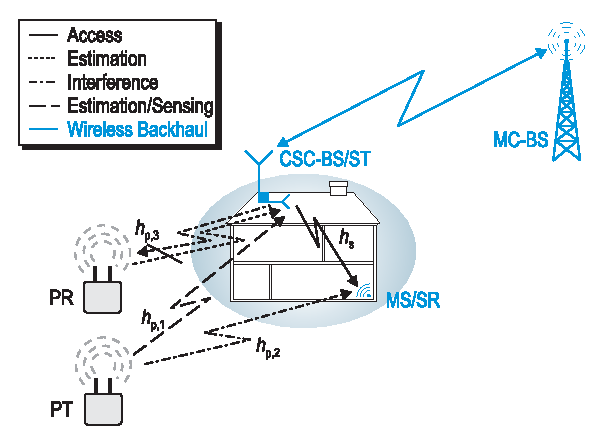
\includegraphics[width = \figscalet]{figures/CR_Scenario_Hybrid}
\caption{A cognitive small cell scenario demonstrating: (i) the CR systems employed at the CSC-BS, (ii) the associated network elements, which constitute Cognitive Small Cell-Base Station/Secondary Transmitter (CSC-BS/ST), Mobile Station/Secondary Receiver (MS/SR), Macro Cell-Base Station (MC-BS) and Primary Transmitter (PT), (iii) the interacting channels: sensing ($\hpo$), interference ($\hptw, \hpth$) and access ($\hs$) channels.}
\label{fig:scenario}
%\vspace{-6mm}
\end{figure}


In context with a CR system, the channel knowledge, unlike conventional or state-of-the-art wireless systems, is not confined to a single transmitter-receiver link, rather it includes all the related channels that exist within as-well-as across the primary and the secondary systems, cf. \figurename~\ref{fig:scenario}. The channels' knowledge is paramount to the CR systems, since it allows them to exercise different techniques, cf. \figurename~\ref{fig:paradigm}, and to obey the desired constraints. Besides, the performance of the CR systems also depends on the channels between these two systems. In absence of this knowledge, especially of those channels that are related to the interference at the primary systems, renders the performance characterization of a CR system incomplete and inadequate for the practical implementations. Despite the existence of multitude of analytical models in the literature (ISs -- \cite{Liang08, Sharma14, Pradhan15}, USs -- \cite{Xing07, Ghasemi07, Kang09}, HSs -- \cite{Song13, Gmira15, Jiang13, Fili15}) that consider with the performance analysis of a CR system, its performance with regard to the channel estimation, due to the complexity of the problem, has never been completely understood\footnote{In context to the US, certain works \cite{Musa09, Suraweera10, Kim12} have dealt with the issue of channel estimation in a CR system, however, unlike this thesis, the investigation has not been exhaustive. This issue is extensively outlined in chapter \ref{chap:US} under the section related work.}. In order to curtail this gap, this thesis capitalizes on the estimation of the involved channels in a CR system. The accessibility of the channel knowledge at the CSC-BS enables the implementation of the CR techniques at the CSC-BS, and allows it perform shared access by establishing a CR communication link with the MS over the acquired spectrum so that the desired level of interference at the PR is not exceeded. 

Certainly, an access to the channels' knowledge comes at a certain cost. Firstly, the inclusion of channel estimation demands an allocation of a certain time interval by the CSC-BS. In consideration to the time allocation, a certain degradation in the performance in terms of the throughput is obvious. Secondly, the variations introduced due to the estimation process, also treated as imperfect channel knowledge leads to an uncertainty in the interference defined as \textit{uncertain interference}\footnote{The uncertain here symbolizes the interference that exists only because of the imperfect channel knowledge, which is not dealt in the literature.} to the primary systems. If not considered, this uncertain interference may severely degrade the performance of the CR systems. In order to approach a successful integration of channel estimation into the CR system, it is essential to consider the performance degradation due to the time allocation and the uncertain interference in the system model, which are not addressed in the existing models that consider the perfect knowledge of the involved channels. This thesis takes these effects into account to establish analytical frameworks (each for the IS, the US and the HS) that allow us to understand the behaviour of the CR systems under those situations that are much closer to the realistic scenarios. %Subsequently, these frameworks are utilized to characterize the performance of the respective CR systems. 

Shifting the focus back to the deployment, it is worthy to understand that the secondary access to the licensed spectrum is viable only if the CR system is equipped with the knowledge about to the primary system, thus, it is dependent on the wireless standard followed by the primary system. This signifies that a preliminary processing in the form of synchronization and demodulation of the baseband signal received from the primary system is necessary. The existence of multiple wireless standards and their complexity preclude us from deploying a dedicated circuitry corresponding to each primary system \cite{Ghasemi08_cm}. Under these circumstances, it is advisable to consider only those solutions that offer low complexity and show versatility towards different primary user signals. Generally speaking, such solutions will not only ease the deployment process but also has a large acceptance among the community. For instance, energy based detection (or energy detection) has been a popular choice compared to its counterparts such as matched-filtering and cyclo-stationary based detection for detecting a PU signal, required for performing spectrum sensing for the interweave systems (discussed later in chapter \ref{chap:IS}). A direct comparison of these techniques by counting their implementations for hardware demonstration has been done in \cite{Pawe11}. 

On similar grounds as energy detection, in order to approach the channel estimation for the CR system, particularly for the channels that involve the primary systems, a \textit{received power-based} channel estimation technique is proposed as a part of the analytical framework in the thesis. This technique is introduced for substituting the conventional techniques such as training-based \cite{Stoica03}, pilot-based \cite{Gifford05, Gifford08}, signal to noise ratio-based \cite{Chav11, Sharma13} channel estimation, which already exist in the literature, because, like energy detection, employing received power-based estimation assures the low complexity and the versatility towards unknown primary user signal requirements of the CR system and consequently facilitates its deployment. Besides, the channel within the secondary framework, treated as a conventional transmitter-receiver link, does not fall in the aforementioned category. Therefore, its knowledge is procured by employing a pilot-based channel estimation technique.

\ifdebug
\begin{figure}
        \centering
        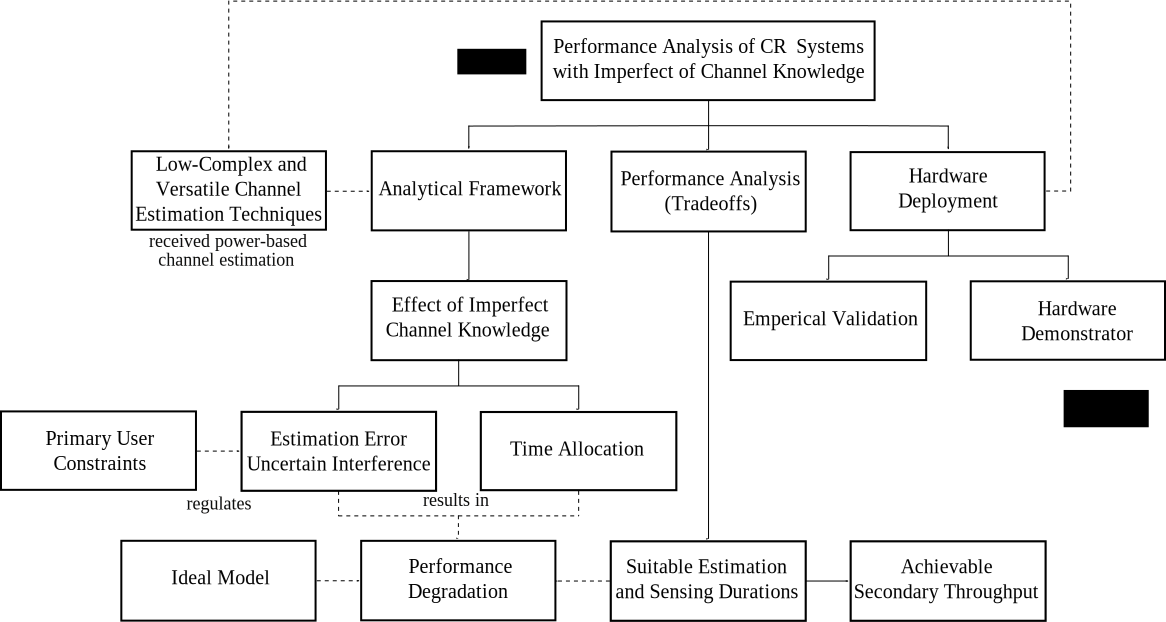
\includegraphics[width=\textheight]{figures/Contri}
        \caption{An illustration of the interconnect between the major contributions and the key observations.}
        \label{fig:contri}
\end{figure}
\else
\begin{sidewaysfigure}
        \centering
        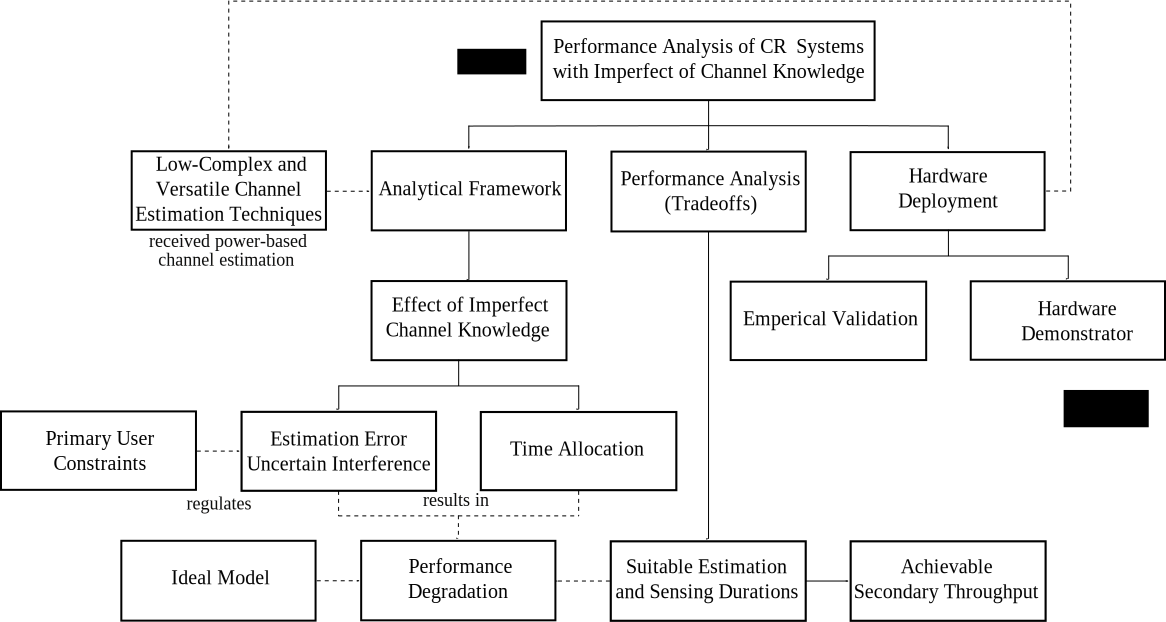
\includegraphics[width=\textheight]{figures/Contri}
        \caption{An illustration of the interconnect between the major contributions and the key observations.}
        \label{fig:contri}
\end{sidewaysfigure}
\fi

\section{Main Contributions}
At this stage, it is well-recognized that the knowledge of the related channels is crucial for the application of CR techniques in practical scenarios. In order to facilitate the hardware deployment of a CSC, a CR application, this thesis capitalizes on the successful integration of this knowledge for different CR systems, namely interweave systems, underlay system and hybrid systems. In this context, the main contributions and the observations of this thesis (also presented in \figurename~\ref{fig:contri}) are summarized as follows:
\begin{itemize}
\item \textit{Analytical Framework}: 
As a major contribution, this thesis proposes an analytical framework, corresponding to the different CR systems (which are followed in chapter \ref{chap:IS}, chapter \ref{chap:US} and chapter \ref{chap:HS}, respectively), that incorporates the estimation of the involved channels between the primary and the secondary systems, a crucial aspect that has been addressed inadequately in the literature. In order to satisfy the low complexity and versatility towards unknown Primary User (PU) signal requirements, which are necessary for the deployment of the CR systems, a received power-based channel estimation is included in the proposed framework. In addition, a careful allocation of the time interval (estimation time), for the purpose of performing channel estimation, in the medium access of the secondary system is proposed. Apart from this, this thesis considers a stochastic approach to tackle the variations in the CR system that arise due to the imperfect channel knowledge (estimation error). In contrast to the existing models that preclude channel estimation (or consider perfect channel knowledge), thereby overestimating the performance of the CR systems, this thesis captures a clear insight on the influence of the time allocation and the imperfect channel knowledge on performance of the CR system. Obviously, such an influence has an detrimental effect on the performance of the CR system, thus, leads to a \textit{performance degradation}. This degradation is qualified through a comparison between the existing models and the estimation model (the one included as a part of the proposed framework). Particularly, the variations cause \textit{uncertain interference} to the primary system, which in some situations could be deleterious to the primary system, are captured by means of novel constraints introduced as the part this framework. In order to closely examine the relationship between the system parameters, theoretical expressions pertaining to the performance analysis of the CR system are derived. Furthermore, to understand the performance of the proposed framework in fading scenarios, especially the interweave and the underlay systems, the analysis is extended to obtain the theoretical expressions that incur the effect of fading in the involved channels. Finally, to exclude any discrepancy in the analysis, the obtained expressions are validated by means of Monte-Carlo simulations. 
\item \textit{Tradeoffs}: 
As a major outcome of the analysis, it has been identified that the estimation time is closely associated with the performance of the CR systems. On one side, it is related to the variations incurred in the system, whereby the level of uncertainty in the interference induced due to the channel estimation in the system can be effectively controlled. While on the other side, it has a great influence on the throughput achieved at the SR. In this thesis, this kind of dual dependency of the performance parameters, classified as the uncertain interference and the secondary throughput (which are individually associated to the performance of primary and secondary system, respectively) on the estimation time has been investigated in the form of tradeoffs, namely \textit{estimation-sensing-throughput} tradeoff for the IS and the HS, and \textit{estimation-throughput} tradeoff for the US. These tradeoffs present a useful tool for visualizing the response of a CR system (in terms of performance) to different choices of the estimation time so that the performance degradation introduced due to the channel estimation can be carefully regulated. In other words, a system designer can utilize these tradeoffs to preclude situations under which the performance degradation becomes intolerable. Conversely, from a theoretical perspective, these tradeoffs can be used to determine a suitable estimation time that yields the maximum achievable throughput while obeying the interference constraints.
 
 
\item \textit{Hardware deployment}: 
In contrast to the theoretical analysis, this thesis lays emphasis on the portability of the analytical framework on a hardware platform. To a great extent, this not only validates the accuracy of the assumptions made while deriving the theoretical expressions but also justifies the applicability of the proposed framework in realistic scenarios. With the implementation of the received power-based estimation technique, this thesis adds further justification to the claims such as the low-complexity and the versatility to unknown PU signals, presented while developing the analytical framework. Considering these facts, a software-defined radio platform is deployed for obtaining the measurements required for the validation process. In order to complement the validation, the theoretical expressions, which include the probability density functions that characterize the variations in the estimated parameters and the performance tradeoff are compared with their empirical counterparts. Besides validation, this thesis presents a demonstrator that certifies the necessity of channels' knowledge for the performance characterization as-well-as for the deployment of a CR system. In this regard, following the guidelines of an US, a demonstrator is deployed. As a part of the deployment process, % to determine the performance of a CR system. As a major outcome of the deployment process, the significance of the channels' knowledge for the performance characterization as-well-as for the deployment, in context with the CR, is justified. %
in order to illustrate a successful deployment of the CR systems, this thesis identifies and discusses some key issues (the ones which are usually left aside while performing the theoretical analysis) and proposes the corresponding simplifications/solutions.  
\end{itemize}

\section{Organization} \todo{Reconsider while revising the individual chapters. Also, update the hyper-links to the Sections below.}

The rest of the chapters in this thesis are organized as follows:

Chapter \ref{chap:IS} develops an analytical framework that incorporates the estimation of involved channels in accordance with the interweave scenario. In this context, the indoor deployment scenario, refer to \figurename~\ref{fig:scenario} is transformed into an interweave scenario, whereby a spectrum sensing mechanism is employed at the CSC-BS enabling a shared (secondary) access to the licensed spectrum. Section 2.4 derives the theoretical expressions that captures the effect of imperfect channel knowledge on the performance. Further, Section 2.5 establishes an estimation-sensing-throughput tradeoff that depicts the suitable estimation and the suitable sensing time at which the maximum throughput is achieved by an IS. 


Following a similar methodology as chapter \ref{chap:IS}, chapter \ref{chap:US} develops an analytical framework that incorporates the estimation of involved channels in accordance to the underlay scenario. To implement the underlay technique within the CSC, the deployment scenario is modified such that a power control mechanism is employed at the CSC-BS so that interference is avoided at the PR. As a part of the proposed framework, Section 3.2 derives the theoretical expressions for the power control and the secondary throughput, which captures the effect of imperfect channel knowledge and characterizes the performance of the US. The performance of a US is jointly characterized in terms of estimation-throughput tradeoff that determines the achievable throughput by an US. 

Despite the interweave and the underlay systems, discussed in the previous chapters (chapter \ref{chap:IS} and chapter \ref{chap:US}), propose different mechanisms (i.e., sensing and power control, respectively) for controlling the interference, individually these systems do not represent the best techniques of utilizing the licensed spectrum efficiently. In this regard, to promote the efficient usage of the licensed spectrum by the secondary users, the underlay and the interweave techniques are combined to realize a hybrid scenario. Motivated by this fact, chapter \ref{chap:HS} develops an analytical framework that incorporates the estimation of involved channels with respect to the hybrid scenario. In this context, the indoor scenario is modified such that the CSC-BS employs spectrum sensing as-well-as power control mechanism to perform secondary access to the licensed spectrum. The theoretical expressions derived in this chapter incorporate the effect of imperfect channel knowledge, and consequently depict the performance of the HS. Analog to chapter \ref{chap:IS}, an estimation-sensing-throughput tradeoff that yields the achievable throughput for the HS is characterized in this chapter. 

 
In order to reveal the ground truth regarding the analysis proposed in previous chapters, chapter \ref{chap:HVD} takes into account the deployment aspects of the proposed framework. In this regard, a hardware that implements the channel estimation, realizes the interference constraints, validates the performance analysis and illustrates the principle working of the US, is deployed.   

Finally, chapter \ref{chap:Con} summarizes the thesis and presents some extensions for the future. 
